\documentclass[10pt,a4paper]{article}

\usepackage[utf8]{inputenc}
\usepackage[T1]{fontenc}
\usepackage{mathptmx}
\usepackage{graphicx}
\usepackage{hyperref}
\usepackage{xcolor}
\usepackage{enumitem}

\makeatletter

\textheight 25.0cm
\topmargin -21mm
\textwidth 17.5cm
\oddsidemargin -5mm
\evensidemargin \oddsidemargin
\pagestyle{empty}
\headsep 13mm

\def\*{{}$^\ast$}
\def\ps@headings{%
      \let\@oddfoot\@empty\let\@evenfoot\@empty
      \def\@evenhead{\@empty}%
      \let\@mkboth\markboth}
\newcommand\mlarge{\@setfontsize\mlarge\@xipt{13.6}}
\def\title#1{\def\@title{#1}}
\def\authors#1{\def\@authors{#1}}
\def\affiliations#1{\def\@affiliations{#1}}
\def\author{\authors}
\def\affiliation{\affiliations}
\def\maketitle{\thispagestyle{headings}\begin{center}
{\mlarge\textbf{\MakeUppercase{\@title}}}\\[13pt]
{\mlarge\@authors}\\
{\mlarge\textit{\@affiliations}}\end{center}}

\newenvironment{summary}
{\small\underline{\textit{Summary}}\ \ }{}

\setcounter{secnumdepth}{0}

\renewcommand\section{\@startsection {section}{1}{\z@}%
                                   {-\baselineskip}%
                                   {\baselineskip}%
                                   {\centering\normalfont\normalsize\bfseries}{\uppercase}}
\renewcommand\subsection{\@startsection {section}{1}{\z@}%
                                   {-\baselineskip}%
                                   {1pt}%
                                   {\normalfont\normalsize\bfseries}{}}
\renewcommand\subsubsection{\@startsection {section}{1}{\z@}%
                                   {-\baselineskip}%
                                   {1pt}%
                                   {\normalfont\normalsize\itshape}{}}
\renewcommand\paragraph{\subsubsection}

\def\@startsection#1#2#3#4#5#6#7{%
  \if@noskipsec \leavevmode \fi
  \par
  \@tempskipa #4\relax
  \ifdim \@tempskipa <\z@
    \@tempskipa -\@tempskipa \@afterindentfalse
  \fi
  \if@nobreak
    \everypar{}%
  \else
    \addpenalty\@secpenalty\addvspace\@tempskipa
  \fi
  \@ifstar
    {\@ssect{#3}{#4}{#5}{#6}{#7}}%
    {\@dblarg{\@sect{#1}{#2}{#3}{#4}{#5}{#6}{#7}}}}

\def\@sect#1#2#3#4#5#6#7[#8]#9{%
  \ifnum #2>\c@secnumdepth
    \let\@svsec\@empty
  \else
    \refstepcounter{#1}%
    \protected@edef\@svsec{\@seccntformat{#1}\relax}%
  \fi
  \@tempskipa #5\relax
  \ifdim \@tempskipa>\z@
    \begingroup
      #6 \hskip #3\relax\@svsec\interlinepenalty \@M #7{#9}\@@par
    \endgroup
  \else
    \def\@svsechd{%
      #6{\hskip #3\relax
      \@svsec #7{#9}}%
    }%
  \fi
  \@xsect{#5}}

\def\@ssect#1#2#3#4#5#6{%
  \@tempskipa #3\relax
  \ifdim \@tempskipa>\z@
    \begingroup
      #4 \hskip #1\interlinepenalty \@M #5{#6}\@@par
    \endgroup
  \else
    \def\@svsechd{#4{\hskip #1\relax #5}}%
  \fi
  \@xsect{#3}}

\long\def\@makecaption#1#2{%
  \vskip\abovecaptionskip
  \sbox\@tempboxa{{\small\textbf{#1.} #2}}%
  \ifdim \wd\@tempboxa >\hsize
    {\small\textbf{#1.} #2}\par
  \else
    \global \@minipagefalse
    \hb@xt@\hsize{\hfil\box\@tempboxa\hfil}%
  \fi
  \vskip\belowcaptionskip}

\def\thebibliography#1{\subsection*{References}\vskip13pt\footnotesize\list
  {\@biblabel{\arabic{enumiv}}}{\settowidth\labelwidth{\@biblabel{#1}}%
    \parsep0pt\itemsep0pt plus 1pt\labelsep1mm\leftmargin7mm\labelwidth6mm
    \usecounter{enumiv}%
    \let\p@enumiv\@empty
    \def\theenumiv{\arabic{enumiv}}}%
    \def\newblock{\hskip .11em plus.33em minus.07em}%
    \sloppy\clubpenalty4000\widowpenalty4000
    \sfcode`\.=1000\relax}

\def\endthebibliography{%
  \def\@noitemerr{\@warning{Empty `thebibliography' environment}}%
  \endlist}

\parindent 0pt
\parskip 1pt plus 0.2pt
\setlist[itemize]{leftmargin=1.2em, topsep=0.2em, itemsep=0.2em}
\hypersetup{colorlinks=true, urlcolor=blue}

\makeatother

\title{Medical Assistant Workflows for Clinical Monitoring, Drug Safety, and Health Risk Support}
\authors{Phuc-Khanh-Nhi NGUYEN$^{1,\ast}$}
\affiliations{$^1$Universit\'e d'\'Evry Paris-Saclay, \'Evry-Courcouronnes, \^Ile-de-France, France.\\Author e-mail: phuckhanhnhi.nguyen@etud.univ-evry.fr}

\begin{document}
\maketitle

\begin{summary}
Modern clinical software increasingly needs to help non-specialist users navigate medication safety questions, vital-sign interpretation, and patient risk assessment without requiring direct interaction with fragmented data tables or backend services. This work presents a medical assistant prototype integrated into a web dashboard and a persistent Python backend. The current system supports five structured workflows: early-warning alerting, drug interaction checking, drug side-effect lookup, health risk prediction from tabular vital-sign inputs, and patient-specific prescription review. Rather than relying on unrestricted generation, the assistant prioritizes deterministic dataset-backed retrieval for medication safety tasks, a pretrained machine-learning model for risk estimation, and guideline retrieval for early-warning alerts. A structured dashboard routes requests through API bridges to backend services that normalize inputs, query local repositories, retrieve guideline context when needed, and return explainable responses. Preliminary implementation results show that this architecture is practical for controlled medical assistance scenarios while preserving a clear boundary between evidence-backed outputs and autonomous diagnosis.
\end{summary}

\section*{Problem Context and Related Work}
Clinical teams and healthcare learners often need rapid support for medication safety questions, side-effect monitoring, early-warning review, and the interpretation of patient risk indicators. In practice, these tasks are still frequently handled by manually consulting separate references, static documents, or spreadsheets, which makes the workflow fragmented and time-consuming. AI-enabled clinical systems can make access to medical information more practical, but purely generative use remains problematic in clinical settings where traceability, consistency, and evidence awareness matter. Our work therefore focuses on a middle ground: a medical assistant that offers a usable dashboard while grounding its main workflows in structured local data, guideline retrieval, and model artifacts.

The aim is not to replace clinical judgment, but to provide practical decision support through concise, evidence-aware outputs. In this sense, the current prototype is intentionally narrow: it targets task types that benefit from deterministic processing while demonstrating how a dashboard-oriented interface can sit on top of medical backend services. This positioning is consistent with prior work on clinical decision support, predictive risk modeling, and medication-focused support systems~\cite{sutton2020,wang2022,muylle2021}. Taken together, these references motivate the present design choice of combining structured task access with bounded, auditable workflows rather than relying on unconstrained medical generation.

\section*{Current System Architecture and Implementation}
The implemented system is organized as a lightweight application stack with a medical dashboard front end, API routes, a persistent Python backend, and workflow-specific services. The web interface provides the main \texttt{/medical} experience, where users submit structured inputs for clinical monitoring and medication safety. Requests are routed through application endpoints to a backend process that dispatches them across specialized workflows.

At the workflow layer, five capabilities are currently implemented:
\begin{itemize}
\item \textbf{Early-warning alerting.} A patient identifier and timestamp are used to retrieve sensor observations and health-record context. Abnormal sensor patterns trigger guideline retrieval and a source-cited early-warning alert for medical staff review.
\item \textbf{Drug interaction checking.} Medication names are normalized, pairwise combinations are generated, and interactions are looked up from a structured local dataset. The system returns only dataset-backed matches, along with source-aware explanations and safety-oriented recommendations.
\item \textbf{Drug side-effect lookup.} One or more normalized drug names are used to retrieve structured side-effect entries from a local repository. Results are displayed separately per medication so that multi-drug queries remain easy to inspect.
\item \textbf{Health risk prediction.} A pretrained logistic-regression model consumes tabular vital-sign features such as respiratory rate, oxygen saturation, systolic blood pressure, heart rate, temperature, consciousness, and oxygen support status. The workflow returns a predicted risk class, confidence score, and top contributing features to support interpretation.
\item \textbf{Patient-specific prescription review.} A patient identifier and medication list are used to check newly prescribed medications against the patient's health record and configured patient-history safety rules.
\end{itemize}

The design uses explicit task-based workflows rather than an unstructured request flow. For medication safety and risk scoring, deterministic services are treated as the primary execution path. Early-warning alerts are the only workflow that uses guideline RAG: abnormal observations are converted into a query, relevant guideline context is retrieved, and the final alert includes citations. This architecture helps separate user-friendly clinical access from the evidence-producing components of the system.

\begin{figure}[t]
\centering
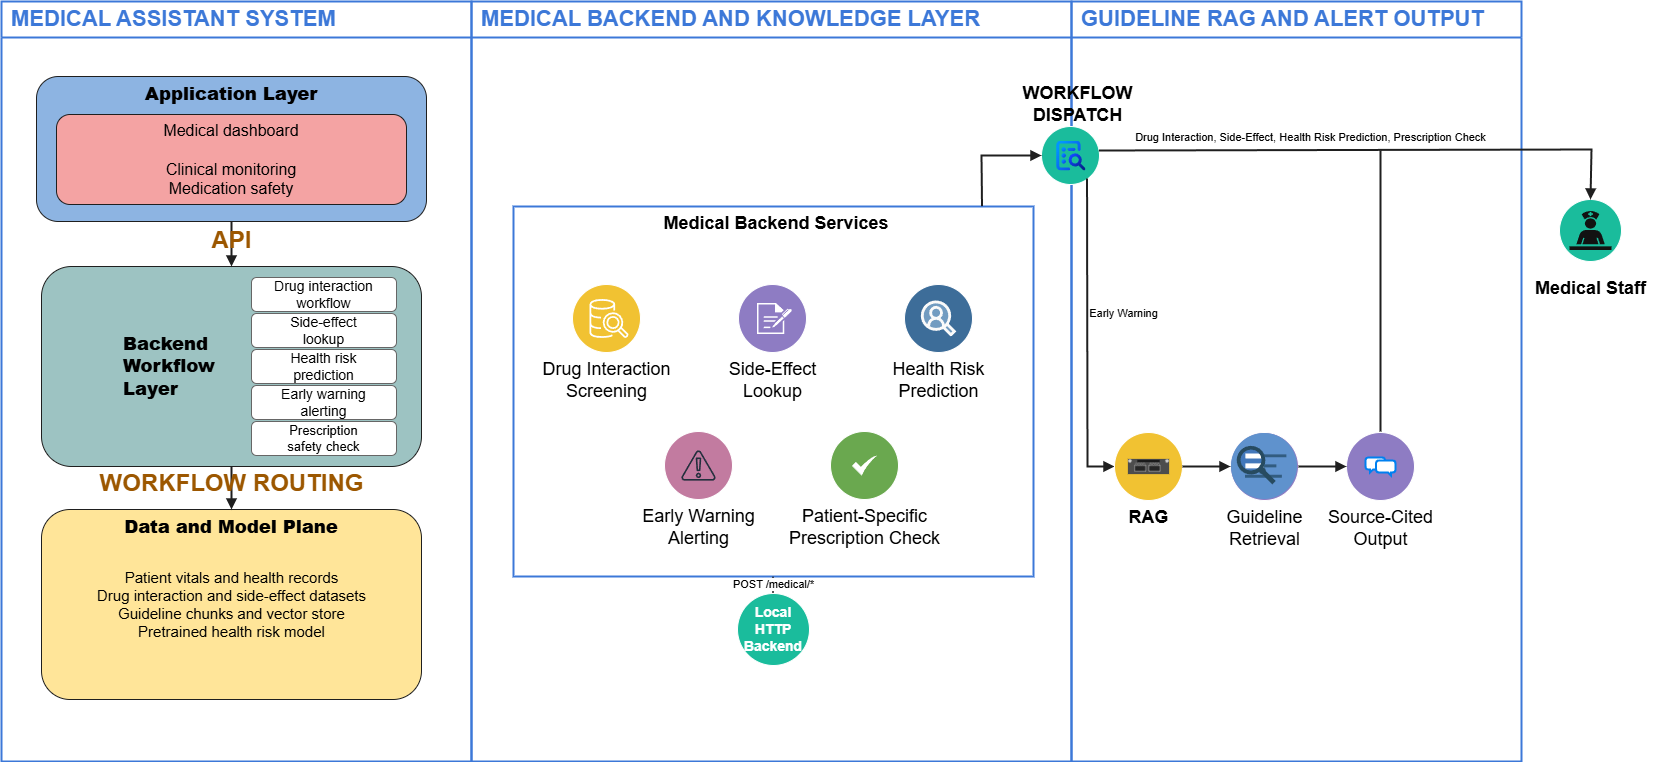
\includegraphics[width=0.90\linewidth]{overview.png}
\caption{Architecture of the current medical assistant prototype, including direct structured outputs for medication-safety and risk workflows, and guideline RAG for early-warning alerts.}
\label{fig:overview}
\end{figure}

\section*{Preliminary Capabilities and Observations}
The current prototype demonstrates that a medical assistant can combine dashboard access with bounded medical workflows without requiring fully generative reasoning at every step. Drug interaction checking is designed as a database-first process, which improves reproducibility because the returned interaction descriptions are tied to explicit structured records. Side-effect lookup similarly benefits from repository-driven outputs, enabling grouped summaries that retain a clear connection to the underlying source text. Health risk prediction extends the system beyond pure lookup by introducing a pretrained classifier that can convert vital-sign profiles into risk categories with basic explanation support. Early-warning alerting adds a guideline-backed branch for abnormal sensor events.

From a systems perspective, this mixed architecture offers two practical advantages. First, it allows a shared interface for multiple medical tasks while preserving specialized processing logic for each task class. Second, it reduces the pressure to rely on a generative model as the sole source of medical truth. This is especially important in an early prototype. For this reason, the current system acts as a controlled task-based medical assistant rather than an autonomous diagnostic system.



\section*{Guideline Retrieval for Early-Warning Alerts}
The retrieval-augmented component is currently used for early-warning alerts rather than free-form diagnosis. When an abnormal sensor pattern is detected, the system generates a clinical query, retrieves relevant guideline chunks, and uses this context to produce a source-cited alert. Other workflows, including drug interaction checking, side-effect lookup, health risk prediction, and patient-specific prescription review, return structured results directly to medical staff.

\section*{Conclusions}
This work presents the current state of a medical assistant prototype that combines dashboard access with structured backend workflows for early-warning alerting, drug interaction checking, side-effect lookup, health risk prediction, and patient-specific prescription review. The implemented architecture demonstrates that it is feasible to integrate local repositories, patient-history lookup, sensor records, guideline retrieval, and a pretrained tabular risk model within a single assistant-oriented system. The present contribution lies less in unrestricted generation and more in the careful orchestration of bounded medical tasks through workflow-specific interfaces.

The current production emphasis remains on deterministic data-backed workflows, guideline-backed early-warning alerts, and explainable model outputs.


\begin{thebibliography}{3}
\bibitem{sutton2020}
Sutton, R. T., Pincock, D., Baumgart, D. C., Sadowski, D. C., Fedorak, R. N., and Kroeker, K. I. An overview of clinical decision support systems: benefits, risks, and strategies for success. \textit{npj Digital Medicine}, 3, Article 17, 2020. DOI: \url{https://doi.org/10.1038/s41746-020-0221-y}.

\bibitem{wang2022}
Wang, Z., Nian, X., and Sun, J. Integrated Convolutional and Recurrent Neural Networks for Health Risk Prediction using Patient Journey Data with Many Missing Values. \textit{arXiv preprint} arXiv:2211.06045, 2022. URL: \url{https://arxiv.org/abs/2211.06045}.

\bibitem{muylle2021}
Muylle, K. M., Gentens, K., Dupont, A. G., and Cornu, P. Evaluation of an optimized context-aware clinical decision support system for drug-drug interaction screening. \textit{International Journal of Medical Informatics}, 152, 104393, 2021. DOI: \url{https://doi.org/10.1016/j.ijmedinf.2021.104393}.
\end{thebibliography}

\end{document}
